\begin{ccRefFunction}{compare_y_at_x}

\ccFunction{Comparison_result compare_y_at_x(const Point_2<Kernel> &p,
                                             const Line_2<Kernel> &h);}
        {compares the $y$-coordinates of $p$ and the vertical projection
         of \ccStyle{p} on \ccStyle{h}%
         \ccTexHtml{ (Figure~\ref{fig-compare2} (d))}{, see (d) in the figure 
         below}.
         \ccPrecond \ccStyle{h} is not vertical.
         }

 \begin{ccTexOnly}
\begin{figure}[h]
\centerline{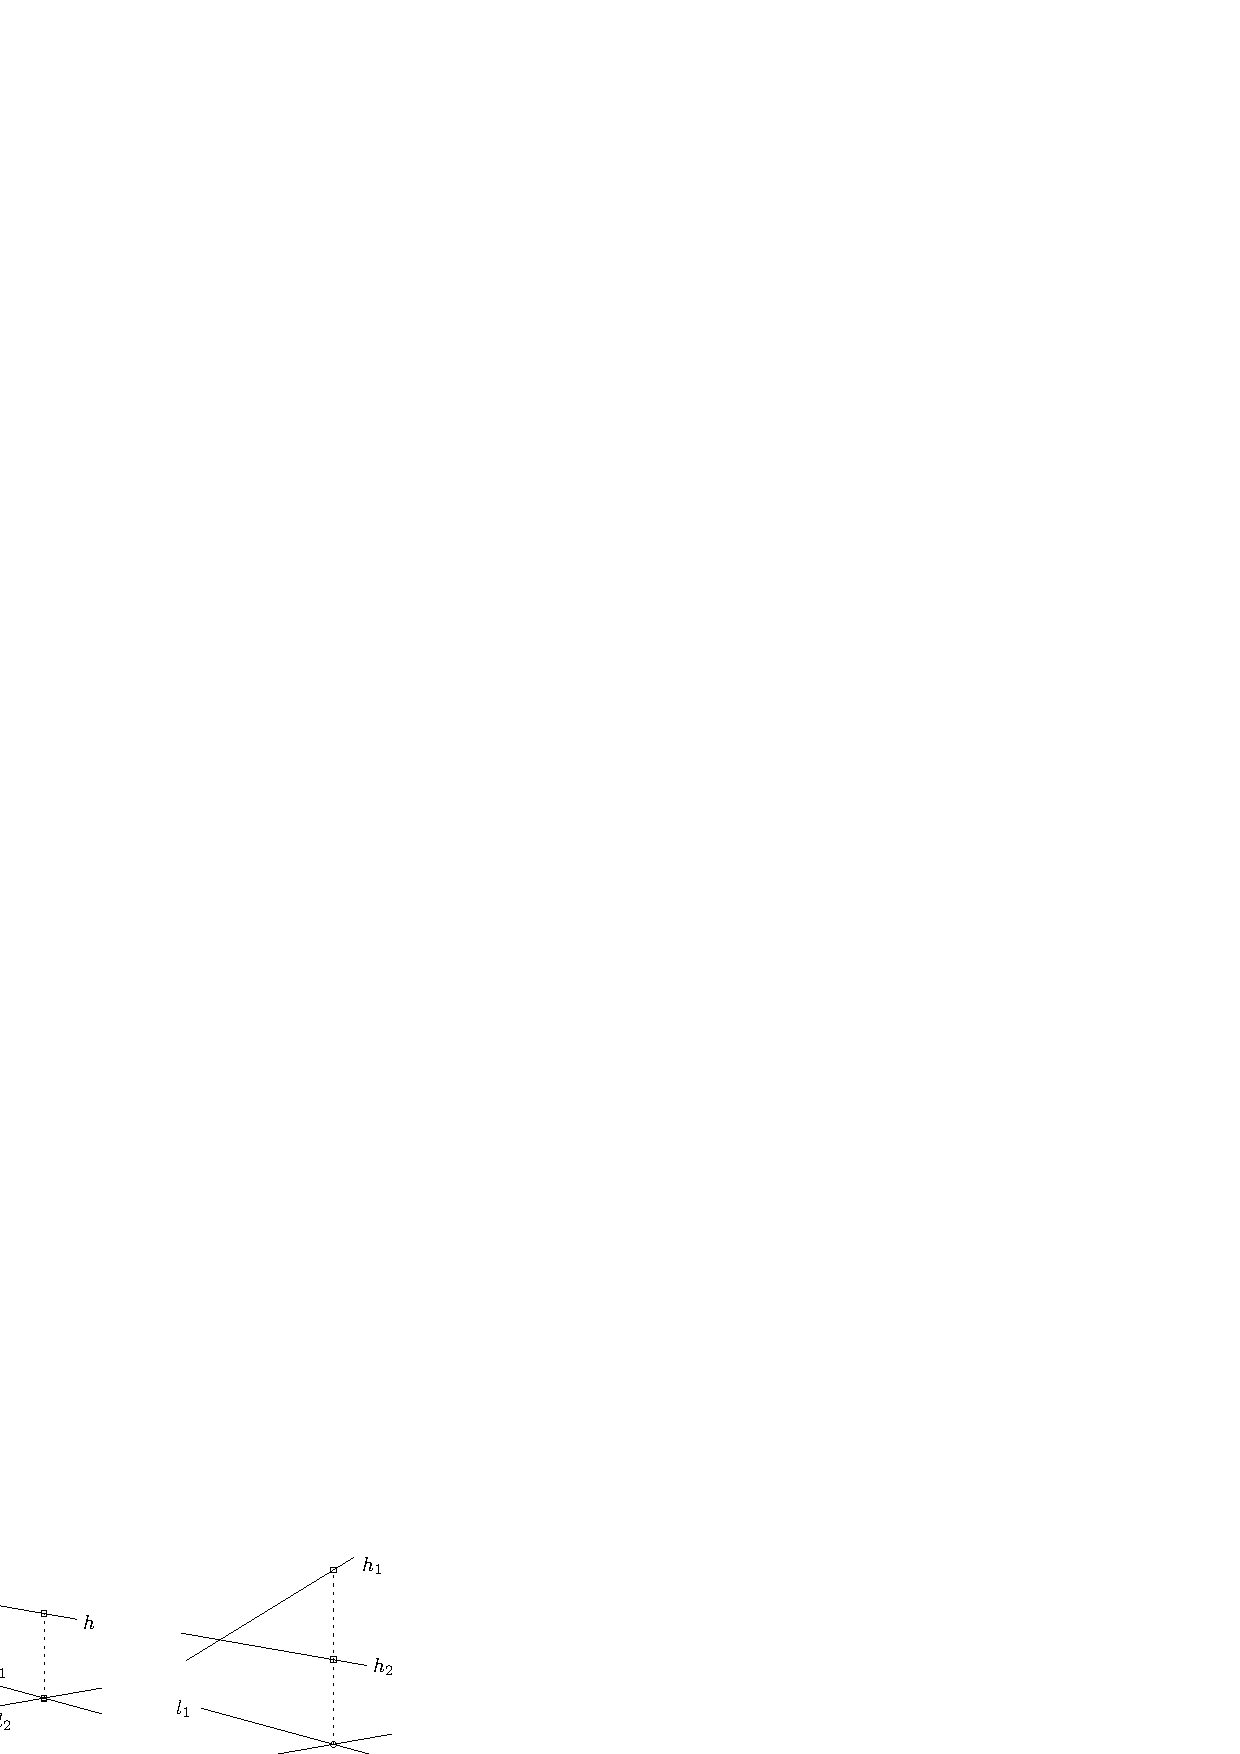
\includegraphics{Kernel_23_ref/fig/compare2}}
\caption{Comparison of the $y$-coordinates of the (implicitly given)
         points in the boxes, at an $x$-coordinate. The $x$-coordinate
         is either given explicitly (disc) or implicitly (circle).
         \label{fig-compare2}}
\end{figure} 
\end{ccTexOnly} 

\ccFunction{Comparison_result compare_y_at_x(const Point_2<Kernel> &p,
                                           const Line_2<Kernel> &h1,
                                           const Line_2<Kernel> &h2);}
{compares the $y$-coordinates of the vertical projection 
 of \ccStyle{p} on \ccStyle{h1} and on \ccStyle{h2}%
 \ccTexHtml{ (Figure~\ref{fig-compare2} (e))}{, see (e) in the figure 
 below}.
\ccPrecond \ccStyle{h1} and \ccStyle{h2} are not vertical.
}


\ccFunction{Comparison_result compare_y_at_x(const Line_2<Kernel> &l1,
                                           const Line_2<Kernel> &l2,
                                           const Line_2<Kernel> &h);}
      {Let $p$ be the \ccHtmlNoLinksFrom{intersection} of lines $l1$ and $l2$.
       This function compares the $y$-coordinates of $p$ and 
       the vertical projection of \ccStyle{p} on \ccStyle{h}%
       \ccTexHtml{ (Figure~\ref{fig-compare2} (f))}{, see (f) in the figure 
       below}.
       \ccPrecond \ccStyle{l1}, \ccStyle{l2} intersect and \ccStyle{h} is not
       vertical.
      }


\ccFunction{Comparison_result compare_y_at_x(const Line_2<Kernel> &l1,
                                           const Line_2<Kernel> &l2,
                                           const Line_2<Kernel> &h1,
                                           const Line_2<Kernel> &h2);}
{Let $p$ be the \ccHtmlNoLinksFrom{intersection} of lines $l1$ and $l2$. This function 
 compares the $y$-coordinates of the vertical projection of \ccStyle{p} on 
 \ccStyle{h1} and on \ccStyle{h2}%
 \ccTexHtml{ (Figure~\ref{fig-compare2} (g))}{, see (g) in the figure 
 below}.
 \ccPrecond \ccStyle{l1} and \ccStyle{l2} intersect; \ccStyle{h1} and 
 \ccStyle{h2} are not vertical.
}

\ccFunction{Comparison_result compare_y_at_x(const Point_2<Kernel> &p,
                                             const Segment_2<Kernel> &s);}
{compares the $y$-coordinates of $p$ and the vertical projection
 of \ccStyle{p} on \ccStyle{s}.  If \ccc{s} is vertical, then return
 \ccc{EQUAL} when \ccc{p} lies on \ccc{s}, \ccc{SMALLER} when \ccc{p} lies
 under {s}, and \ccc{LARGER} otherwise.
 \ccPrecond \ccStyle{p} is within the x range of \ccStyle{s}.}

\ccFunction{Comparison_result compare_y_at_x(const Point_2<Kernel> &p,
                                           const Segment_2<Kernel> &s1,
                                           const Segment_2<Kernel> &s2);}
{compares the $y$-coordinates of the vertical projection 
 of \ccStyle{p} on \ccStyle{s1} and on \ccStyle{s2}.  If \ccc{s1} or \ccc{s2}
 is vertical, then return \ccc{EQUAL} if they intersect, otherwise return
 \ccc{SMALLER} if \ccc{s1} lies below \ccc{s2}, and return \ccc{LARGER}
 otherwise.
 \ccPrecond \ccStyle{p} is within the x range of \ccStyle{s1} and \ccStyle{s2}.}


\begin{ccHtmlOnly}
<img border=0 src="fig/compare2.gif" align=middle alt="Comparison of y at x">
\end{ccHtmlOnly} 

\ccSeeAlso
\ccRefIdfierPage{CGAL::compare_xy} \\
\ccRefIdfierPage{CGAL::compare_xyz} \\
\ccRefIdfierPage{CGAL::compare_x} \\
\ccRefIdfierPage{CGAL::compare_x_at_y} \\
\ccRefIdfierPage{CGAL::compare_y} \\
\ccRefIdfierPage{CGAL::compare_yx} \\
\ccRefIdfierPage{CGAL::compare_z} \\

\end{ccRefFunction}

